\input{regression-test.tex}
\documentclass[degree=bachelor]{thuthesis}

\thusetup{
  title      = {本科生综合论文训练标题},
  department = {计算机科学与技术系},
  discipline = {计算机科学与技术},
  author     = {某某某},
  supervisor = {某某某, 教授},
  date       = {2024-11-01},
}

\usepackage[sort]{natbib}


\begin{document}
\START
\showoutput

\maketitle

\copyrightpage

\frontmatter

\begin{abstract}
  论文的摘要是对论文研究内容和成果的高度概括。摘要应对论文所研究的问题及其研究目的进行描述,
  对研究方法和过程进行简单介绍,对研究成果和所得结论进行概括。
  摘要应具有独立性和自明性,其内容应包含与论文全文同等量的主要信息。使读者即使不阅读全文,
  通过摘要就能了解论文的总体内容和主要成果。

  论文摘要的书写应力求精确、简明。切忌写成对论文书写内容进行提要的形式,尤其要避免“第1章……;
  第2章……;……”这种或类似的陈述方式。

  关键词是为了文献标引工作、用以表示全文主要内容信息的单词或术语。
  每篇论文应选取3~5个关键词,每个关键词中间用分号分隔。

  \thusetup{
    keywords = {关键词1, 关键词2, 关键词3, 关键词4, 关键词5},
  }
\end{abstract}


\begin{abstract*}
  An abstract of a dissertation is a summary and extraction of research work and con-tributions.
  Included in an abstract should be description of research topic and research ob-jective, brief introduction to methodology and research process, and summarization of conclusion and contributions of the research.
  An abstract should be characterized by inde-pendence and clarity and carry identical information with the dissertation.
  It should be such that the general idea and major contributions of the dissertation are conveyed without reading the dissertation.

  An abstract should be concise and to the point.
  It is a misunderstanding to make an abstract an outline of the dissertation and words “the first chapter”, “the second chapter” and the like should be avoided in the abstract.

  Keywords are terms used in a dissertation for indexing, reflecting core information of the dissertation.
  The number of keywords should be between 3 and 5, with semi-colons used in between to separate one another.

  \thusetup{
    keywords* = {word 1, keyword 2, keyword 3, keyword 4, keyword 5},
  }
\end{abstract*}


\tableofcontents

\listoffigures

\listoftables

\begin{denotation}[6.8em]
  \item[$a$, $c_1$, $c_2$] 临时替换变量
  \item[$D_{\text{m}}$] 预混通道外径 (mm)
  \item[Ga] 空气质量流量 (kg/s)
  \item[Ma] 进口空气马赫数,$\text{Ma} = \nu_2 / \gamma R T_2$
  \item[$\gamma$] 比热比=1.4
  \item[$\delta$] 总压损失系数,$\delta = \increment p_{2-3} / p_2$ (\%)
  \item[$\varphi_{\text{LLO}}$] 贫燃着火极限
  \item[CFD] 计算流体力学 (Computational Fluid Dynamics)
  \item[DFT] 密度泛函理论 (Density Functional Theory)
  \item[LBO] 贫燃熄火极限 (Lean Blowout Value)
  \item[ONIOM] 分层算法 (Our own N-layered Integrated molecular Orbital and molecular Mechanics)
  \item[PES] 势能面 (Potential Energy Surface)
  \item[PIV] 颗粒图像速度仪 (Particle Image Velocimetry)
  \item[SCF] 自洽场 (Self-Consistent Field)
  \item[SCRF] 自洽反应场 (Self-Consistent Reaction Field)
  \item[TS] 过渡态 (Transition State)
  \item[TST] 过渡态理论 (Transition State Theory)
  \item[ZPE] 零点振动能 (Zero Vibration Energy)
\end{denotation}


\mainmatter

\chapter{引言}

\section{一级节标题第一条}

此部分是论文主体部分的文字格式示例。

\subsection{二级节标题第一条}

主体部分一般从引言(绪论)开始,以结论结束。

引言(绪论)应包括论文的研究目的、流程和方法等。

论文研究领域的历史回顾,文献回溯,理论分析等内容,应独立成章,用足够的文字叙述。

主体部分由于涉及的学科、选题、研究方法、结果表达方式等有很大的差异,不能作统一的规定。
但是,必须实事求是、客观真切、准确完备、合乎逻辑、层次分明、简练可读。


\subsection{二级节标题第二条}

论文中应引用与研究主题密切相关的参考文献。
参考文献的写法应遵循国家标准《信息与文献 参考文献著录规则》(GB/T 7714—2015);
符合特定学科的通用范式,可使用APA或《清华大学学报(哲学社会科学版)》格式,
且应全文统一,不能混用。此处是正文中引用参考文献的上标标注示例[1]。

当论文中的字、词或短语,需要进一步加以说明,而又没有具体的文献来源时,用注释。
注释一般在社会科学中用得较多。应控制论文中的注释数量,不宜过多。
由于论文篇幅较长,建议采用文中编号加“脚注”的方式。此处是脚注格式规范示例
\footnote{%
  脚注处序号“①,……,⑩”的字体是“正文”,不是“上标”,
  序号与脚注内容文字之间空半个汉字符,脚注的段落格式为:单倍行距,段前空0磅,段后空0磅,
  悬挂缩进1.5字符;字号为小五号字,汉字用宋体,外文用Times New Roman体。
}。



\chapter{图、表及表达式示例}

\section{论文中图的示例}

图应具有“自明性”,即只看图、图题和图例,不阅读正文,就可理解图意。示例如下:

\begin{figure}[h]
  \centering
  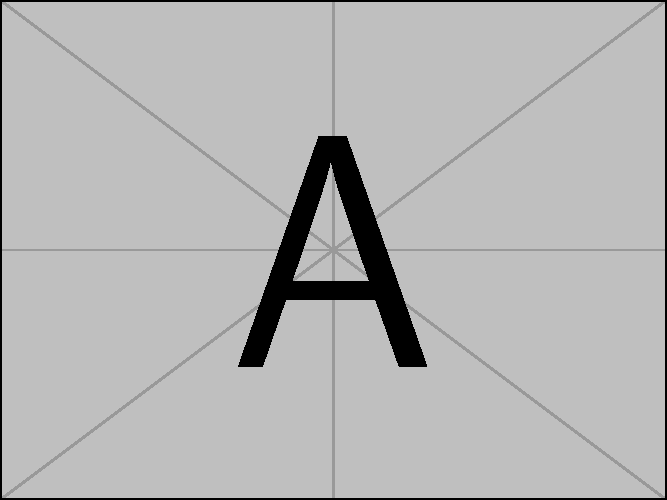
\includegraphics[height=6.7cm]{example-image-a.pdf}
  \caption{不同光源照射30分钟后测定的紫菌样品紫外-可见吸收光谱}
  \label{fig:example-1}
\end{figure}


\section{论文中表的示例}

表应具有“自明性”。表的编排,一般是内容和测试项目由左至右横读,数据依序竖读。示例如下:

\begin{table}[h]
  \centering
  \caption{字体、字型、字号及段落格式要求}
  \label{tab:example-1}
  \begin{tabular}{cccc}
    & 文字举例 & 中文字体、字号要求 & 英文及数字字体、字号要求 \\
    章标题 & 第1章 引言 & 黑体三号字 & Arial三号 \\
    一级节标题 & 4.1 标题示例 & 黑体四号字 & Arial 14pt \\
    二级节标题 & 3.2.2 标题示例 & 黑体13pt字 & Arial 13pt \\
    三级节标题 & 5.3.3.2 标题示例 & 黑体小四号字 & Arial 12pt \\
  \end{tabular}
\end{table}

\clearpage


\section{论文中表达式的示例}

表达式主要是指数字表达式,例如数学表达式,也包括文字表达式。示例如下:
\begin{equation}
  \mathrm{NH}_4^+ + 2\mathrm{O}_2 \rightarrow \mathrm{NO}_2^- + \mathrm{H}_2 \mathrm{O} + 2 \mathrm{H}^+
\end{equation}



\nocite{*}
\citestyle{thuthesis-bachelor}

\begin{thebibliography}{8}
\providecommand{\natexlab}[1]{#1}
\providecommand{\url}[1]{#1}
\expandafter\ifx\csname urlstyle\endcsname\relax\else
  \urlstyle{same}\fi
\expandafter\ifx\csname href\endcsname\relax
  \DeclareUrlCommand\doi{\urlstyle{rm}}
  \def\eprint#1#2{#2}
\else
  \def\doi#1{\href{https://doi.org/#1}{\nolinkurl{#1}}}
  \let\eprint\href
\fi

\bibitem[竺可桢(1973)]{zhukezhen1973}
竺可桢.
\newblock 物理学\allowbreak[M].
\newblock 北京: 科学出版社, 1973: 56-60.

\bibitem[胡楚雄(2024)]{huchuxiong2024jicheng}
胡楚雄, 周冉, 付宏, 等.
\newblock 集成电路装备光刻机发展前沿与未来挑战\allowbreak[J].
\newblock 中国科学: 信息科学, 2024, 54(1): 130-143.
\newblock DOI: \doi{10.1360/SSI-2023-0378}.

\bibitem[Hu et~al.(2020)]{hu2020}
HU C, OU T, CHANG H, et al.
\newblock Deep GRU Neural Network Prediction and Feedfor-ward Compensation for Precision Multiaxis Motion Control Systems\allowbreak[J].
\newblock IEEE-ASME Transactions on Mechatronics, 2020, 25(3): 1377-1388.

\bibitem[Weinstein et~al.(1974)Weinstein and Swertz]{weinstein1974pathogenic}
WEINSTEIN L, SWERTZ M~N.
\newblock Pathogenic properties of invading
  microorganism\allowbreak[M]//\allowbreak
SODEMAN W~A, Jr, SODEMAN W~A.
\newblock Pathologic physiology: mechanisms of disease.
\newblock Philadelphia: Saunders, 1974: 745-772.

\bibitem[郑开青(1987)]{zhengkaiqing1987}
郑开青.
\newblock 通讯系统模拟及软件\allowbreak[D].
\newblock 北京: 清华大学无线电系, 1987.

\bibitem[胡楚雄(1987)]{huchuxiong2024zhixian}
胡楚雄, 汪泽, 付宏.
\newblock 直线电机装置及其重力补偿组件: ZL202210922042.5\allowbreak[P].
\newblock 2024-06-04.

\bibitem[中华人民共和国国家技术监督局(1987)]{zhonghua1994}
中华人民共和国国家技术监督局.
\newblock GB3100-3102. 中华人民共和国国家标准-量与单位\allowbreak[S].
\newblock 北京: 中国标准出版社, 1994.

\bibitem[傅刚\ 等(2000)傅刚, 赵承, and 李佳路]{fugang2000fengsha}
傅刚, 赵承, 李佳路.
\newblock 大风沙过后的思考\allowbreak[N/OL].
\newblock 北京青年报, 2000-04-12\allowbreak (14)\allowbreak[2002-03-06].
\newblock \url{http://www.bjyouth.com.cn/Bqb/20000412/B/4216%5ED0412B1401.htm}.

\end{thebibliography}


\appendix
\begin{translation}

\title{调研阅读报告题目}
\maketitle

写出至少 5000 外文印刷字符的调研阅读报告或者书面翻译 1~2 篇(不少于 2 万外文印刷符)。

\vspace{20bp}%

\citestyle{thuthesis-bachelor}
\begin{thebibliography}{1}
\bibitem[某某某(1994)]{mou1994}
某某某.
\newblock 信息技术与信息服务国际研讨会论文集: A 集[C].
\newblock 北京:中国社会科学出版社,1994.
\end{thebibliography}

\end{translation}


\backmatter

\begin{acknowledgements}
  衷心感谢指导教师××教授对本人的精心指导。他的言传身教将使我终生受益。

  感谢×××××实验室××教授,以及×××××全体老师和同窗们的热情帮助和支持!

  ……

  本课题承蒙×××××基金资助,特此致谢。
\end{acknowledgements}


\statement


\begin{resume}
  \section*{学术论文}

  \begin{achievements}
    \item ZHOU R, HU C, OU T, et al. Intelligent GRU-RIC Position-Loop
      Feedforward Compensation Control Method with Application to an
      Ultraprecision Motion Stage[J], IEEE Transactions on Industrial
      Informatics, 2024, 20(4): 5609-5621.

    \item 杨轶, 张宁欣, 任天令, 等. 硅基铁电微声学器件中薄膜残余应力的研究[J].
      中国机械工程, 2005, 16(14):1289-1291.

    \item YANG Y, REN T L, ZHU Y P, et al. PMUTs for handwriting recognition.
      In press[J]. (已被Integrated Ferroelectrics录用)

  \end{achievements}


  \section*{专利}

  \begin{achievements}
    \item 胡楚雄, 付宏, 朱煜, 等. 一种磁悬浮平面电机: ZL202011322520.6[P]. 2022-04-01.

    \item REN T L, YANG Y, ZHU Y P, et al. Piezoelectric micro acoustic sensor
      based on ferroelectric materials: No.11/215, 102[P]. (美国发明专利申请号.)

  \end{achievements}
\end{resume}


\clearpage
\OMIT
\end{document}
